%\documentclass[12pt,spanish,fleqn,openany,letterpaper,pagesize]{scrbook}

\usepackage[utf8]{inputenc}
\usepackage[spanish]{babel}
\usepackage{fancyhdr}
\usepackage{epsfig}
\usepackage{epic}
\usepackage{eepic}
\usepackage{amsmath}
\usepackage{threeparttable}
\usepackage{amscd}
\usepackage{here}
\usepackage{graphicx}
\usepackage{lscape}
\usepackage{tabularx}
\usepackage{subfigure}
\usepackage{longtable}


\usepackage{rotating} %Para rotar texto, objetos y tablas seite. No se ve en DVI solo en PS. Seite 328 Hundebuch
                        %se usa junto con \rotate, \sidewidestable ....


\renewcommand{\theequation}{\thechapter-\arabic{equation}}
\renewcommand{\thefigure}{\textbf{\thechapter-\arabic{figure}}}
\renewcommand{\thetable}{\textbf{\thechapter-\arabic{table}}}


\pagestyle{fancyplain}%\addtolength{\headwidth}{\marginparwidth}
\textheight22.5cm \topmargin0cm \textwidth16.5cm
\oddsidemargin0.5cm \evensidemargin-0.5cm%
\renewcommand{\chaptermark}[1]{\markboth{\thechapter\; #1}{}}
\renewcommand{\sectionmark}[1]{\markright{\thesection\; #1}}
\lhead[\fancyplain{}{\thepage}]{\fancyplain{}{\rightmark}}
\rhead[\fancyplain{}{\leftmark}]{\fancyplain{}{\thepage}}
\fancyfoot{}
\thispagestyle{fancy}%


\addtolength{\headwidth}{0cm}
\unitlength1mm %Define la unidad LE para Figuras
\mathindent0cm %Define la distancia de las formulas al texto,  fleqn las descentra
\marginparwidth0cm
\parindent0cm %Define la distancia de la primera linea de un parrafo a la margen

%Para tablas,  redefine el backschlash en tablas donde se define la posici\'{o}n del texto en las
%casillas (con \centering \raggedright o \raggedleft)
\newcommand{\PreserveBackslash}[1]{\let\temp=\\#1\let\\=\temp}
\let\PBS=\PreserveBackslash

%Espacio entre lineas
\renewcommand{\baselinestretch}{1.1}

%Neuer Befehl f\"{u}r die Tabelle Eigenschaften der Aktivkohlen
\newcommand{\arr}[1]{\raisebox{1.5ex}[0cm][0cm]{#1}}

%Neue Kommandos
\usepackage{Befehle}


%Trennungsliste
\hyphenation {Reaktor-ab-me-ssun-gen Gas-zu-sa-mmen-set-zung
Raum-gesch-win-dig-keit Durch-fluss Stick-stoff-gemisch
Ad-sorp-tions-tem-pe-ra-tur Klein-schmidt
Kohlen-stoff-Mole-kular-siebe Py-rolysat-aus-beu-te
Trans-port-vor-gan-ge}

%
%\begin{document}

\chapter{Motivación y objetivos}


\justifying
\section{Motivación}

  \par El mosquito es uno de los vectores de enfermedades humanas más importantes
    en el mundo. En particular, el \textit{Aedes aegypti} es el principal vector
    de Dengue, Chikungunya, Zika y Fiebre Amarilla urbana \cite{dengue_principal}.
    Según datos de la Organización Mundial de la Salud (OMS), alrededor de 80 millones de
    personas se infectan de Dengue anualmente, cerca de 550 mil enfermos requieren hospitalización y
    unos 20 mil mueren. Además, calculan que más de 2.500 millones de personas corren
    riesgo de contraer la enfermedad y más de 100 países tienen transmisión endémica
    \cite{directices_ministerio}.
    Cabe aclarar que en el caso de la Fiebre Amarilla existe una vacuna de virus
    atenuado que se considera eficaz para la prevención, segura
    y se la utiliza hace más de 60 años en la inmunización activa de niños y
    adultos. Para el Dengue, Chikungunya y Zika,
    no existe tal herramienta de previsión.

  \par \textit{Médicos del Mundo}\footnote{http://www.mdm.org.ar}, en su nota
    \textbf{"Médicos del Mundo alerta sobre riesgos de fiebre amarilla en Brasil y escenarios de Dengue-Zika en Argentina"}
    explican que entre 1985 y 2012, si tenemos en cuenta las cuatro enfermedades
    mencionadas en el párrafo anterior, en las Américas el 95\% de los casos se concentraron en
    4 países: Perú (54\% de los casos), Bolivia (18\%), Brasil (16\%) y Colombia (7\%).
    También dicen que, aún así, Argentina, Ecuador, Panamá y Venezuela también tienen condiciones
    muy favorables para la transmisión.



  \par En el caso de Argentina, para el año 2016, podemos observar la taza de
  Dengue a nivel
  provincia \cite{analisis_cordoba} en la
  Figura \ref{fig:dengue}\footnote{Figura brindada por Rotela y
  colaboradores de su trabajo \cite{analisis_cordoba}.}, a su vez desde la
  emergencia del virus del Zika en nuestro país en el mismo año (Tucumán),
  y hasta el 2017 se registraron además un total de 7 casos confirmados de
  síndrome congénito asociados a virus del Zika en mujeres embarazadas
  (microcefalia en recién nacidos).
  Durante el 2017, en base a las notificaciones al
  \textbf{Sistema Nacional de Vigilancia de Salud} del Ministerio de Salud de la Nación
  recibidas hasta el 30 de diciembre, se registraron, en el primer semestre del año, brotes de
  Dengue serotipo DEN-1 con 646 casos confirmados en cinco provincias
  (Buenos Aires, Chaco, Corrientes, Formosa y Santa Fe) y 253 casos de enfermedad
  por virus del Zika en tres provincias (Chaco, Formosa y Salta).
  Incluso ya para las primeras semanas del 2018, hubo casos confirmados
  de Dengue en Chaco.

  \begin{figure}
  \centering%
  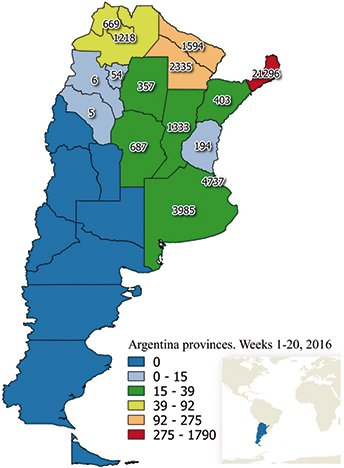
\includegraphics[width=0.4\textwidth]{images/dengue}%
  \caption{La taza de Dengue en Argentina a nivel provincia en 2016.
          Dicha taza es expresada cada 100.000 habitantes; se tienen en cuenta
          todos los casos confirmados y probables hasta la semana 20.}\label{fig:dengue}
  \end{figure}


  \par El Dr. Gonzalo Basile \footnote{Presidente Honor y Director General para
                   América Latina y Caribe de Médicos del Mundo, e investigador de institutos de
                   investigación en salud pública del Caribe y coordinación regional del Programa
                   de Salud Internacional de CLACSO y de FLACSO República Dominicana.}
       se refiere al incremento del riesgo de crecimiento
       en la cantidad de casos positivos en nuestro país, teniendo en cuenta
       el contexto epidemiológico en la región:
    \begin{framed}

      Aunque las últimas epidemias del 2009 y 2016 de Dengue en Argentina fueron del
      serotipo DEN1, la circulación viral de los otros serotipos en la región de
      Cono Sur (Brasil, Paraguay y Bolivia) tanto DEN4, DEN2 y DEN3, hace que los
      periodos epidémicos de DEN se puedan modificar. Por otro lado, el escenario de
      Zika Virus es una realidad por su circulación en América Latina y Caribe con
      cuadros clínicos inéspecíficos pero con eventos asociados como el Síndrome de
      Guillaen Barré y microcefalia que implican problemas epidemiológicos
      poblacionales de incidencia como lo demostraron en Brasil, Colombia, Venezuela,
      República Dominicana, entre otros 47 países de la región donde se confirmaron
      casos de transmisión activa vectorial de Zika.
      Si sumamos ahora el brote epidémico de Fiebre Amarilla en Brasil con la
      posibilidad de reintroducir casos en el Cono Sur ya que las tasas de
      inmunizaciones para fiebre amarrilla existen brechas en varias ciudades de nuestro país. \textbf{24/01/2018}
    \end{framed}



  \par Sumado a lo comentado, por su parte, el \textit{Aedes aegypti} se
    caracteriza por su presencia en el medio urbano, su preferencia
    de cría en contenedores artificiales \cite{cont_artificiales} y la
    resistencia de sus huevos a la
    desecación. En nuestro país, además, los vertiginosos cambios demográficos, han dado
    por resultado una gran ampliación desorganizada de las zonas urbanas. Ésto, junto
    con el aumento del uso de recipientes no biodegradables y un método deficiente
    de recolección de residuos sólidos, incrementan el número de depósitos que
    acumulan agua, que actúan como potenciales criaderos del mosquito, lo cual aumenta el
    riesgo de ocurrencia de casos de las enfermedades mencionadas.
    Dado que la cantidad de vectores, el virus circulante y la susceptibilidad
    humana dependen directa o indirectamente de variables climáticas y ambientales
    tales como la temperatura, la lluvia, la vegetación, entre otras,
    el cambio climático es, también, un factor de riesgo para el desarrollo
    de las enfermedades en cuestión. Por otra parte, se le suma la capacidad adaptativa del
    \textit{Aedes aegypti} y la aparición de resistencia del mismo debido al uso intensivo de
    insecticidas.


  \par Por otro lado, como se menciona anteriormente, dado que no hay vacunas para la
    mayoría de estos virus, y existe la posibilidad de introducción de otros \cite{emergencia_viral},
    el control de vectores es la principal herramienta para mitigar la
    propagación de enfermedades.


  \par Es claro que el escenario epidémico planteado es una realidad en Argentina
    que hay que atacar. Ésto deriva en la necesidad de enfocar esfuerzos en el
    desarrollo de estrategias contundentes dirigidas a evitar, limitar y controlar
    las poblaciones de \textit{Aedes aegypti}, lo que implica repensar y diseñar
    nuevos sistemas de alerta temprana, vigilancia epidemiológica y respuesta
    rápida desde lo local, integrando un espacio interinstitutional e
    intersectorial de coordinación, planificación e intervención pública. Ésto debe
    llevarse a cabo entre el Estado Nacional, municipios, universidades y centros
    de estudio, organizaciones civiles, entre otros actores sociales de gran importancia.
    En ese contexto, la introducción de herramientas científico/tecnológicas orientadas
    a contribuir en esos aspectos resulta fundamental.

  \par El uso de información satelital se ha estado utilizando desde hace
    algunos años, como uno de los métodos para atacar el problema mencionado.
    Ésta técnica permite modelar la evolución temporal y geográfica de las
    poblaciones del vector utilizando variables ambientales obtenidas de los
    sensores remotos. Aunque hasta ahora, estos trabajos utilizaban fuertes suposiciones
    al utilizar modelos lineales para relacionar las distintas variables, y por más
    que los resultados obtenidos hasta el momento han sido
    favorables, no existen resultados que prueben el hecho de que las
    relaciones que se establecen entre el desarrollo
    del mosquito y las variables ambientales del entorno son de tipo lineal.
    Esto nos permite generar la hipótesis de que modelos no-lineales son
    capaces de modelar relaciones que se adapten mejor a la realidad.
    Una de las formas de probarla es utilizar modelos no-lineales de
    aprendizaje automático para llevar a cabo esa tarea.


  \par Desarrollar un modelo de aprendizaje automático puede resultar extremadamente
    complejo y costoso en términos computacionales y de experiencia de quien lo lleve
    a cabo. Uno de los objetivos de este trabajo es mostrar la accesibilidad,
    en términos de simpleza y costos, de algunas de estas herramientas, sin dejar
    de lado el desempeño en la tarea concreta. A su vez, también existe el importante problema
    de la escasez de datos de campo para utilizarlos en la construcción de los modelos.
    Hasta ahora, era un gran limitante ya que no se tienen datos vitales
    para el desarrollo de este tipo de herramientas. En este trabajo, además, se
    propone una técnica para atenuar dicho problema estableciendo una relación
    entre los distintos puntos geográficos, en función de sus características ambientales.

\section{Objetivos}

  \par Los objetivos del trabajo apuntan a aportar conocimientos y
    herramientas a los profesionales dedicados al desarrollo de sistemas de
    prevención y mitigación del Dengue, Zika, Chikungunya y enfermedades
    vectoriales en general. Para ello, se establecen los siguientes puntos
    a desarrollar:
    \begin{itemize}
      \item Implementación de una herramienta para la generación de nuevos modelos
        predictivos a partir de variables ambientales. Dadas las
        características interdisciplinarias de la
        problemática en la epidemiología, dicha herramienta
        debe ser utilizable por profesionales que no sean expertos en
        informática o en aprendizaje automático.
      \item Validar la hipótesis de que modelos no-lineales son mejores
        para predecir y ajustar la oviposición de mosquitos que los modelos
        lineales utilizados hasta el momento.
      \item Proponer una solución a la problemática de la
        escasez de puntos con datos de campo para entrenar los modelos,
        dada la naturaleza regional de un sistema de riesgo, que aporte a
        valor los existentes.
    \end{itemize}

%\end{document}
